\documentclass[a4paper,12pt]{article}
\usepackage[brazil]{babel} 
\usepackage[utf8]{inputenc} 

\usepackage{amssymb}
\usepackage{algorithm}
\usepackage{algpseudocode}

\usepackage{indentfirst} 
\usepackage{listings}
\usepackage{graphicx}
\usepackage{url}

\begin{document} 



\begin{titlepage}

\newcommand{\HRule}{\rule{\linewidth}{0.5mm}} % Defines a new command for the horizontal lines, change thickness here

\center % Center everything on the page
 
%----------------------------------------------------------------------------------------
%	HEADING SECTIONS
%----------------------------------------------------------------------------------------

\textsc{\LARGE Universidade Federal\\do Espírito Santo}\\[1.5cm] % Name of your university/college
\textsc{\Large Centro Tecnológico}\\[0.5cm] % Major heading such as course name
\textsc{\large Departamento de Informática}\\[0.5cm] % Minor heading such as course title

%----------------------------------------------------------------------------------------
%	TITLE SECTION
%----------------------------------------------------------------------------------------

\HRule \\[0.4cm]
{ \huge \bfseries O Problema do Caixeiro Viajante}\\[0.4cm] % Title of your document
\HRule \\[1.5cm]

%----------------------------------------------------------------------------------------
%	AUTHOR SECTION
%----------------------------------------------------------------------------------------

\begin{minipage}{0.4\textwidth}
\begin{flushleft} \large
\emph{Autor:}\\
Vinicius \textsc{Arruda} % Your name
\end{flushleft}
\end{minipage}
~
\begin{minipage}{0.4\textwidth}
\begin{flushright} \large
\emph{Professora:} \\
Mariella \textsc{Berger} % Supervisor's Name
\end{flushright}
\end{minipage}\\[2cm]

% If you don't want a supervisor, uncomment the two lines below and remove the section above
%\Large \emph{Author:}\\
%John \textsc{Smith}\\[3cm] % Your name

%----------------------------------------------------------------------------------------
%	DATE SECTION
%----------------------------------------------------------------------------------------

{\large 02 de Setembro de 2015}\\[2cm] % Date, change the \today to a set date if you want to be precise

%----------------------------------------------------------------------------------------
%	LOGO SECTION
%----------------------------------------------------------------------------------------


\includegraphics[width=58mm]{LogoUfes.png}\\[1cm] % Include a department/university logo - this will require the graphicx package

%----------------------------------------------------------------------------------------

\vfill % Fill the rest of the page with whitespace

\end{titlepage}





\begin{abstract}
Trabalho da disciplina de Estrutura de Dados II, que consiste na implementação 
de quatro soluções diferentes para o Problema do Caixeiro Viajante. As soluções 
são os algoritmos de solução ótima, heurística do vizinho mais próximo, heurística 
de melhoramento 2-opt e heurística do envoltório convexo.
\end{abstract}

%\begin{figure}[hb!]
%\centering
%\includegraphics[width=140mm]{hilbert.jpg}
%\caption{Hilbert.}
%\end{figure}
%\hspace{1.5em}Imagem gerada a partir do interpretador desenvolvido.

\newpage






\section{Introdução} % Este comando faz o tíıtulo da seção.
%INTRODUÇÃO

O Problema do Caixeiro Viajante (do inglês: \textit{Traveling Salesman Problem}, abreviado por TSP) compõe um clássico da 
carreira de algoritmos, teoria dos grafos, otimização combinatória e tantas outras 
áreas de estudos computacionais e matemáticos. Além disso, é um problema fascinante e 
pertence ao seleto grupo de problemas NP-Completo.

O TSP foi inspirado no problema de um vendedor que gostaria de percorrer o menor caminho possível 
saindo de sua cidade atual, passando por diversas cidades vendendo seus produtos e retornando à cidade de origem. 
O TSP pode ser aplicado à diversas áreas, desde problemas de roteamento à criptografia. 

A idéia central destas implementações de soluções para o TSP é mostrar que não é um problema trivial, 
pois para encontrar a solução ótima de \emph{n} cidades é necessário examinar \emph{n - 1} rotas distintas.

A complexidade de tempo em busca da solução ótima é fatorial. Se essa complexidade fosse expressa em termos 
de um polinômio em \emph{n}, os computadores atuais teriam a capacidade de suportar o aumento de \emph{n}.

Das soluções, três delas implementam o Problema do Caixeiro Viajante Assimétrico 
(do inglês: \textit{Asymmetric Traveling Salesman Problem}, abreviado por ATSP) que é uma variante do TSP, 
com a única diferença que a distância de uma cidade A para a cidade B não é a mesma distância 
da cidade B para a cidade A. A única solução que implementa o TSP é a heurística do envoltório convexo. 

Para a implementação das soluções, foram utilizados estruturas de dados estáticas, como vetor e matriz, 
e estruturas de dados dinâmicas, como lista encadeada e pilha.

Por questão de simplicidade, este trabalho utilizará a abreviação TSP para se referir à ambos os problemas e quando 
for necessário enfatizar se há ou não simetria entre as distâncias das cidades, será utilizado \emph{TSP simétrico} e 
\emph{TSP assimétrico}.


%OBJETIVO:
\section{Objetivo}
Aplicar o conhecimento adquirido na disciplina de Estruturas de Dados II para implementar algoritmos 
de melhoramento e heurísticas para encontrar soluções aproximadas para o TSP.
Adquirir conhecimento da complexidade que é solucionar o problema do TSP e a importância que as heurísticas 
possuem para a computação.

%FERRAMENTAS:
\section{Ferramentas}
Os algoritmos foram implementados na linguagem de programação C. Para a compilação foi 
utilizado o compilador GCC versão 4.7.2 em uma máquina com o sistema operacional Debian 
GNU/Linux 7.8 (wheezy).
O código foi escrito utilizando o editor de texto gedit versão 3.4.2.
Para a depuração do programa, foi utilizado a ferramenta Valgrind versão 3.7.0.

%EXATO:
\section{Algoritmo Exato}
O algoritmo \emph{exato} possui solução ótima, porém a complexidade de tempo cresce em escala fatorial em relação 
ao número de cidades. Sua implementação se baseia em analisar o custo de cada caminho possível, e retornar o caminho 
que tiver o menor custo.

\subsection{Metodologia}
O algoritmo \emph{exato} foi implementado utilizando recursão. A figura \ref{Diagrama Exato} mostra o processo de geração de caminhos com 
um exemplo de 4 cidades, partindo da cidade 0. 

\begin{figure}[h!]
\centering
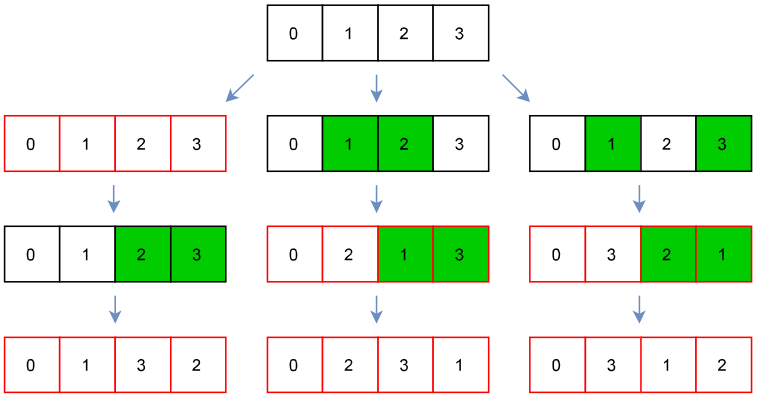
\includegraphics[width=140mm]{ExatoDiagramPng.png}
\caption{Exemplo de execução da implementação para 4 cidades.} \label{Diagrama Exato}
\end{figure}

Na figura \ref{Diagrama Exato}, está marcado em verde as posições do vetor de caminho que irão realizar a troca. Em vermelho estão os diferentes 
caminhos que foram gerados ao longo da execução. Para cada um destes caminhos, é calculado seu custo, e se for o menor custo encontrado até o momento, 
este se torna o custo mínimo atual e o menor caminho atual.

Ao executar o algoritmo \emph{exato}, a pilha de execução irá crescer até \emph{n} chamadas recursivas, onde \emph{n} 
é o número de cidades do TSP. Um problema possível de ocorrer é o estouro da pilha de execução caso \emph{n} seja grande demais, 
porém, se torna inviável  calcular o TSP com um grande número de cidades, pois como já dito anteriormente, o tempo 
de execução cresce em escala fatorial.

%AVALIAÇÃO E RESULTADOS:
\subsection{Avaliação e Resultados}
Para a avaliação do algoritmo \emph{exato} foi utilizado a base de dados \emph{br17}. Esta base 
de dados foi reduzida para as dimensões de 2 à 16, eliminando a última linha e a última coluna para reduzir uma dimensão da base. 
A avaliação foi feita utilizando a função \emph{time} disponível por linha de comando nos sitemas linux.
A tabela \ref{TabelaExato} mostra o resultado obtido.

\begin{table}[H]
\centering
\caption{Resultado da execução do algoritmo exato.} \label{TabelaExato}
\begin{tabular}{ccc}
\hline
Número de cidades & Tempo & Custo do caminho \\
\hline
2       & 0.412s    & 10      \\
3       & 0.432s        & 11      \\
4       & 0.424s     & 104     \\
5       & 0.424s     & 104     \\
6       & 0.416s      & 70      \\
7       & 0.416s      & 36      \\
8       & 0.416s      & 39      \\
9       & 0.468s      & 39      \\
10      & 0.668s      & 39      \\
11      & 2.888s      & 39      \\
12      & 26.470s      & 39      \\
13      & 5m 24.864s      & 39      \\
14      & 67m 31.385s      & 39      \\
15      & 982m 12.383s      & 39      \\
\hline
\end{tabular}
\end{table}



%NN:
\section{Algoritmo NN}
O algoritmo do vizinho mais próximo ou \emph{NN} (abreviação do inglês: \textit{Nearest Neighbor}) pertence à 
classe dos algoritmos gulosos, e tem como funcionamento incluir ao caminho a cidade mais próxima da atual. 


\subsection{Metodologia}
O algoritmo \emph{NN}, partindo de uma cidade inicial, verifica a distância da cidade atual em relação à todas as 
cidades ainda não visitadas e inclui em seu caminho a cidade que houver a menor distância. Isso se repete até que 
todas as cidades estejam no caminho.
O algoritmo \ref{AlgoritmoNN} descreve o algoritmo \emph{NN}.

\begin{algorithm}[H]
\caption{Algoritmo NN} \label{AlgoritmoNN}
\begin{algorithmic}[1]
\Procedure{nn}{}

\State $j \gets 0$
\State $P \gets \varnothing$
\State $P_j \gets initial city$
\State $C \gets C - initial city$

\While{$C \neq \varnothing$} 

\State $min \gets \textit{max}(\textit{distance}(P_j, C))$

\ForAll{$e \in C$}

\If {$\textit{distance}(P_j, e) < min$}
\State $min \gets \textit{distance}(P_j, e)$
\State $temp \gets e$
\EndIf
\EndFor

\State $j \gets j + 1$
\State $P_j \gets e$
\State $C \gets C - e$

\EndWhile
\EndProcedure

\end{algorithmic}
\end{algorithm}


%AVALIAÇÃO E RESULTADOS:
\subsection{Avaliação e Resultados}
Para a avaliação do algoritmo \emph{NN} foi utilizado as bases \emph{ft53.atsp}, \emph{ft70.atsp}, \emph{rbg358.atsp} e \emph{rbg443.atsp}.
A avaliação foi feita utilizando a função \emph{time} disponível por linha de comando nos sitemas linux.
A tabela \ref{TabelaNN} mostra o resultado obtido.

\begin{table}[H]
\centering
\caption{Resultado da execução do algoritmo NN.} \label{TabelaNN}
\begin{tabular}{ccc}
\hline
Número de cidades & Tempo & Custo do caminho \\
\hline
53       & 0.000s    & 9514      \\
70       & 0.000s        & 43186      \\
358       & 0.012s     & 1812     \\
443       & 0.024s    & 3922     \\
\hline
\end{tabular}
\end{table}


%OPT:
\section{Algoritmo 2-opt}
A heurística de melhoramento \emph{2-opt}, é um algoritmo de otimização que faz uma busca local apenas 
verificando possíveis trocas de caminhos entre 4 das \emph{n} cidades do problema.

Neste trabalho, o algoritmo \emph{2-opt} é aplicado sobre um caminho gerado pelo algoritmo \emph{NN}, visando otimizar 
o caminho encontrado, reduzindo seu custo.


\subsection{Metodologia}
O algoritmo \emph{2-opt} percorre o caminho das cidades e para cada par de caminho entre uma cidade e outra, ou seja, para cada par de arestas, 
que não sejam adjacentes, é feita a inversão destes caminhos e verifica se o custo do caminho diminuiu. Ao final de todos os pares de arestas 
possíveis, realiza-se a inversão de caminhos entre as cidades que obtiveram menor custo.


%AVALIAÇÃO E RESULTADOS:
\subsection{Avaliação e Resultados}
Para a avaliação do algoritmo \emph{2-opt} foi utilizada as mesmas bases utilizada para o algoritmo \emph{NN}.
A avaliação foi feita utilizando a função \emph{time} disponível por linha de comando nos sitemas linux.
A tabela \ref{TabelaOPT} mostra o resultado obtido.

\begin{table}[H]
\centering
\caption{Resultado da execução do algoritmo 2-opt.} \label{TabelaOPT}
\begin{tabular}{ccc}
\hline
Número de cidades & Tempo & Custo do caminho \\
\hline
53       & 0.008s    & 8833      \\
70       & 0.016s        & 42490      \\
358       & 3.596s     & 1774     \\
443       & 3.460s    & 3892     \\
\hline
\end{tabular}
\end{table}


Comparando a tabela \ref{TabelaNN} com a \ref{TabelaOPT}, notamos que houve uma melhora do custo do caminho encontrado 
aplicando o algoritmo \emph{2-opt} em uma solução do algoritmo \emph{NN} para as bases de testes acima.



%HULL:
\section{Algoritmo Convex Hull}
O algoritmo \emph{Convex Hull}, é um algoritmo de aproximação que gera uma solução para o TSP em dois passos. O primeiro 
passo é gerar o envoltório convexo, que é um caminho entre as cidades mais externas de maneira que englobe todas as que não 
estejam no caminho do envoltório. O segundo passo, é apartir do caminho gerado pelo envoltório convexo, incluir as cidades que 
não estão no envoltório de maneira que o custo do desvio do caminho para passar nesta cidade seja mínimo.

% figura de cidades, do lado figura do envoltorio e do lado a solução a partir do envoltorio


\subsection{Metodologia}
O algoritmo \emph{Convex Hull} possui várias maneiras de ser implementado. A implementação deste trabalho segue os seguintes
passos:

\begin{enumerate}
\item Considerando as cidades como pontos no plano cartesiano, ordena esses pontos em ordem crescente em relação ao eixo x.
\item Cria a parte superior do envoltório convexo.
\item Cria a parte inferior do envoltório convexo.
\end{enumerate}

Com o envoltório pronto, segue a construção do caminho completo:

\begin{enumerate}
\item Coloca as cidades que estão no envoltório convexo no caminho.
\item \label{Passo1} Para cada cidade que não esteja no caminho (\textit{out}), calcula-se o custo do desvio: \textit{dist(in[i], out) + dist(out, in[i+1]) - dist(in[i], in[i+1])}, onde \textit{in[i]} é a \textit{iésima} cidade pertencente ao caminho.
\item A cidade que possuir o menor custo de desvio é incluída no caminho. \label{Passo2}
\item Enquanto houver cidade fora do caminho, repete o passo \ref{Passo1} e \ref{Passo2}.
\end{enumerate}




%AVALIAÇÃO E RESULTADOS:
\subsection{Avaliação e Resultados}
Para a avaliação do algoritmo \emph{Convex Hull} foi utilizado a base berlin52.tsp.
A avaliação foi feita utilizando a função \emph{time} disponível por linha de comando nos sitemas linux.
A tabela \ref{TabelaCH} mostra o resultado obtido.

\begin{table}[H]
\centering
\caption{Resultado da execução do algoritmo Convex Hull.} \label{TabelaCH}
\begin{tabular}{ccc}
\hline
Número de cidades & Tempo & Custo do caminho \\
\hline
52       & 0.004s    & 8430.44      \\
\hline
\end{tabular}
\end{table}





%REFERÊNCIAS BIBLIOGRÁFICAS:
\section{Referências Bibliográficas}
\begin{enumerate}
\item \url{http://www.mat.ufrgs.br/~portosil/caixeiro.html}
\item \url{https://pt.wikipedia.org/wiki/Complexidade_de_tempo}
\item \url{http://www.iwr.uni-heidelberg.de/groups/comopt/software/TSPLIB95/atsp/}
\item \url{http://tex.stackexchange.com} 
\item \url{http://www.inf.ufes.br/~mberger/Disciplinas/2015_2/EDII/trab1.pdf}
\item \url{http://www.inf.ufes.br/~mberger/Disciplinas/2015_2/EDII/03.pdf}
\item \url{https://en.wikibooks.org/wiki/LaTeX/Algorithms}
\end{enumerate}


\end{document}



